% Created by tikzDevice version 0.10.1 on 2016-08-29 22:52:15
% !TEX encoding = UTF-8 Unicode
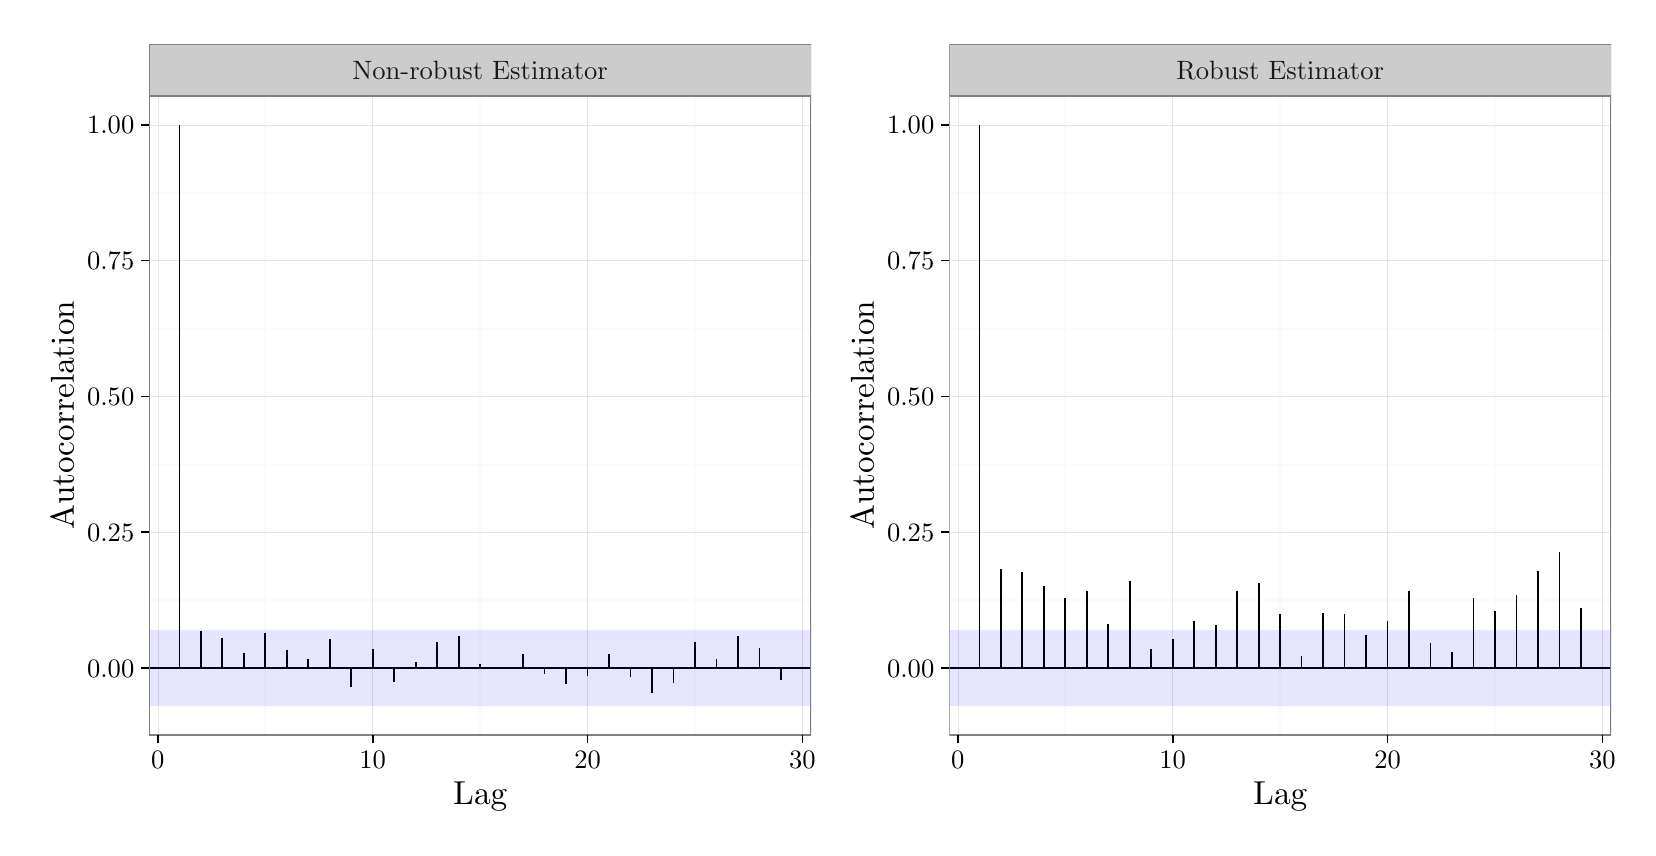
\begin{tikzpicture}[x=1pt,y=1pt]
\definecolor{fillColor}{RGB}{255,255,255}
\path[use as bounding box,fill=fillColor,fill opacity=0.00] (0,0) rectangle (578.16,289.08);
\begin{scope}
\path[clip] (  0.00,  0.00) rectangle (289.08,289.08);
\definecolor{drawColor}{RGB}{255,255,255}
\definecolor{fillColor}{RGB}{255,255,255}

\path[draw=drawColor,line width= 0.6pt,line join=round,line cap=round,fill=fillColor] (  0.00,  0.00) rectangle (289.08,289.08);
\end{scope}
\begin{scope}
\path[clip] ( 43.93, 33.48) rectangle (283.08,264.47);
\definecolor{fillColor}{RGB}{255,255,255}

\path[fill=fillColor] ( 43.93, 33.48) rectangle (283.08,264.47);
\definecolor{drawColor}{gray}{0.98}

\path[draw=drawColor,line width= 0.6pt,line join=round] ( 43.93, 82.19) --
	(283.08, 82.19);

\path[draw=drawColor,line width= 0.6pt,line join=round] ( 43.93,131.27) --
	(283.08,131.27);

\path[draw=drawColor,line width= 0.6pt,line join=round] ( 43.93,180.35) --
	(283.08,180.35);

\path[draw=drawColor,line width= 0.6pt,line join=round] ( 43.93,229.43) --
	(283.08,229.43);

\path[draw=drawColor,line width= 0.6pt,line join=round] ( 85.86, 33.48) --
	( 85.86,264.47);

\path[draw=drawColor,line width= 0.6pt,line join=round] (163.50, 33.48) --
	(163.50,264.47);

\path[draw=drawColor,line width= 0.6pt,line join=round] (241.15, 33.48) --
	(241.15,264.47);
\definecolor{drawColor}{gray}{0.90}

\path[draw=drawColor,line width= 0.2pt,line join=round] ( 43.93, 57.65) --
	(283.08, 57.65);

\path[draw=drawColor,line width= 0.2pt,line join=round] ( 43.93,106.73) --
	(283.08,106.73);

\path[draw=drawColor,line width= 0.2pt,line join=round] ( 43.93,155.81) --
	(283.08,155.81);

\path[draw=drawColor,line width= 0.2pt,line join=round] ( 43.93,204.89) --
	(283.08,204.89);

\path[draw=drawColor,line width= 0.2pt,line join=round] ( 43.93,253.97) --
	(283.08,253.97);

\path[draw=drawColor,line width= 0.2pt,line join=round] ( 47.03, 33.48) --
	( 47.03,264.47);

\path[draw=drawColor,line width= 0.2pt,line join=round] (124.68, 33.48) --
	(124.68,264.47);

\path[draw=drawColor,line width= 0.2pt,line join=round] (202.33, 33.48) --
	(202.33,264.47);

\path[draw=drawColor,line width= 0.2pt,line join=round] (279.97, 33.48) --
	(279.97,264.47);
\definecolor{drawColor}{RGB}{0,0,0}

\path[draw=drawColor,line width= 0.6pt,line join=round] ( 43.93, 57.65) -- (283.08, 57.65);

\path[draw=drawColor,line width= 0.6pt,line join=round] ( 54.80,253.97) -- ( 54.80, 57.65);

\path[draw=drawColor,line width= 0.6pt,line join=round] ( 62.56, 71.09) -- ( 62.56, 57.65);

\path[draw=drawColor,line width= 0.6pt,line join=round] ( 70.33, 68.66) -- ( 70.33, 57.65);

\path[draw=drawColor,line width= 0.6pt,line join=round] ( 78.09, 63.26) -- ( 78.09, 57.65);

\path[draw=drawColor,line width= 0.6pt,line join=round] ( 85.86, 70.52) -- ( 85.86, 57.65);

\path[draw=drawColor,line width= 0.6pt,line join=round] ( 93.62, 64.33) -- ( 93.62, 57.65);

\path[draw=drawColor,line width= 0.6pt,line join=round] (101.39, 61.01) -- (101.39, 57.65);

\path[draw=drawColor,line width= 0.6pt,line join=round] (109.15, 68.14) -- (109.15, 57.65);

\path[draw=drawColor,line width= 0.6pt,line join=round] (116.92, 50.96) -- (116.92, 57.65);

\path[draw=drawColor,line width= 0.6pt,line join=round] (124.68, 64.47) -- (124.68, 57.65);

\path[draw=drawColor,line width= 0.6pt,line join=round] (132.44, 52.60) -- (132.44, 57.65);

\path[draw=drawColor,line width= 0.6pt,line join=round] (140.21, 59.90) -- (140.21, 57.65);

\path[draw=drawColor,line width= 0.6pt,line join=round] (147.97, 66.97) -- (147.97, 57.65);

\path[draw=drawColor,line width= 0.6pt,line join=round] (155.74, 69.17) -- (155.74, 57.65);

\path[draw=drawColor,line width= 0.6pt,line join=round] (163.50, 58.98) -- (163.50, 57.65);

\path[draw=drawColor,line width= 0.6pt,line join=round] (171.27, 57.68) -- (171.27, 57.65);

\path[draw=drawColor,line width= 0.6pt,line join=round] (179.03, 62.77) -- (179.03, 57.65);

\path[draw=drawColor,line width= 0.6pt,line join=round] (186.80, 55.45) -- (186.80, 57.65);

\path[draw=drawColor,line width= 0.6pt,line join=round] (194.56, 51.75) -- (194.56, 57.65);

\path[draw=drawColor,line width= 0.6pt,line join=round] (202.33, 54.69) -- (202.33, 57.65);

\path[draw=drawColor,line width= 0.6pt,line join=round] (210.09, 62.60) -- (210.09, 57.65);

\path[draw=drawColor,line width= 0.6pt,line join=round] (217.86, 54.45) -- (217.86, 57.65);

\path[draw=drawColor,line width= 0.6pt,line join=round] (225.62, 48.63) -- (225.62, 57.65);

\path[draw=drawColor,line width= 0.6pt,line join=round] (233.39, 52.20) -- (233.39, 57.65);

\path[draw=drawColor,line width= 0.6pt,line join=round] (241.15, 67.20) -- (241.15, 57.65);

\path[draw=drawColor,line width= 0.6pt,line join=round] (248.92, 60.98) -- (248.92, 57.65);

\path[draw=drawColor,line width= 0.6pt,line join=round] (256.68, 69.34) -- (256.68, 57.65);

\path[draw=drawColor,line width= 0.6pt,line join=round] (264.44, 64.94) -- (264.44, 57.65);

\path[draw=drawColor,line width= 0.6pt,line join=round] (272.21, 53.31) -- (272.21, 57.65);
\definecolor{fillColor}{RGB}{0,0,255}

\path[fill=fillColor,fill opacity=0.10] ( 43.93, 43.98) rectangle (283.08, 71.32);
\definecolor{drawColor}{gray}{0.50}

\path[draw=drawColor,line width= 0.6pt,line join=round,line cap=round] ( 43.93, 33.48) rectangle (283.08,264.47);
\end{scope}
\begin{scope}
\path[clip] ( 43.93,264.47) rectangle (283.08,283.08);
\definecolor{drawColor}{gray}{0.50}
\definecolor{fillColor}{gray}{0.80}

\path[draw=drawColor,line width= 0.2pt,line join=round,line cap=round,fill=fillColor] ( 43.93,264.47) rectangle (283.08,283.08);
\definecolor{drawColor}{gray}{0.10}

\node[text=drawColor,anchor=base,inner sep=0pt, outer sep=0pt, scale=  0.96] at (163.50,270.47) {Non-robust Estimator};
\end{scope}
\begin{scope}
\path[clip] (  0.00,  0.00) rectangle (578.16,289.08);
\definecolor{drawColor}{RGB}{0,0,0}

\node[text=drawColor,anchor=base east,inner sep=0pt, outer sep=0pt, scale=  0.96] at ( 38.53, 54.34) {0.00};

\node[text=drawColor,anchor=base east,inner sep=0pt, outer sep=0pt, scale=  0.96] at ( 38.53,103.42) {0.25};

\node[text=drawColor,anchor=base east,inner sep=0pt, outer sep=0pt, scale=  0.96] at ( 38.53,152.50) {0.50};

\node[text=drawColor,anchor=base east,inner sep=0pt, outer sep=0pt, scale=  0.96] at ( 38.53,201.58) {0.75};

\node[text=drawColor,anchor=base east,inner sep=0pt, outer sep=0pt, scale=  0.96] at ( 38.53,250.66) {1.00};
\end{scope}
\begin{scope}
\path[clip] (  0.00,  0.00) rectangle (578.16,289.08);
\definecolor{drawColor}{RGB}{0,0,0}

\path[draw=drawColor,line width= 0.6pt,line join=round] ( 40.93, 57.65) --
	( 43.93, 57.65);

\path[draw=drawColor,line width= 0.6pt,line join=round] ( 40.93,106.73) --
	( 43.93,106.73);

\path[draw=drawColor,line width= 0.6pt,line join=round] ( 40.93,155.81) --
	( 43.93,155.81);

\path[draw=drawColor,line width= 0.6pt,line join=round] ( 40.93,204.89) --
	( 43.93,204.89);

\path[draw=drawColor,line width= 0.6pt,line join=round] ( 40.93,253.97) --
	( 43.93,253.97);
\end{scope}
\begin{scope}
\path[clip] (  0.00,  0.00) rectangle (578.16,289.08);
\definecolor{drawColor}{RGB}{0,0,0}

\path[draw=drawColor,line width= 0.6pt,line join=round] ( 47.03, 30.48) --
	( 47.03, 33.48);

\path[draw=drawColor,line width= 0.6pt,line join=round] (124.68, 30.48) --
	(124.68, 33.48);

\path[draw=drawColor,line width= 0.6pt,line join=round] (202.33, 30.48) --
	(202.33, 33.48);

\path[draw=drawColor,line width= 0.6pt,line join=round] (279.97, 30.48) --
	(279.97, 33.48);
\end{scope}
\begin{scope}
\path[clip] (  0.00,  0.00) rectangle (578.16,289.08);
\definecolor{drawColor}{RGB}{0,0,0}

\node[text=drawColor,anchor=base,inner sep=0pt, outer sep=0pt, scale=  0.96] at ( 47.03, 21.46) {0};

\node[text=drawColor,anchor=base,inner sep=0pt, outer sep=0pt, scale=  0.96] at (124.68, 21.46) {10};

\node[text=drawColor,anchor=base,inner sep=0pt, outer sep=0pt, scale=  0.96] at (202.33, 21.46) {20};

\node[text=drawColor,anchor=base,inner sep=0pt, outer sep=0pt, scale=  0.96] at (279.97, 21.46) {30};
\end{scope}
\begin{scope}
\path[clip] (  0.00,  0.00) rectangle (578.16,289.08);
\definecolor{drawColor}{RGB}{0,0,0}

\node[text=drawColor,anchor=base,inner sep=0pt, outer sep=0pt, scale=  1.20] at (163.50,  8.40) {Lag};
\end{scope}
\begin{scope}
\path[clip] (  0.00,  0.00) rectangle (578.16,289.08);
\definecolor{drawColor}{RGB}{0,0,0}

\node[text=drawColor,rotate= 90.00,anchor=base,inner sep=0pt, outer sep=0pt, scale=  1.20] at ( 16.66,148.97) {Autocorrelation};
\end{scope}
\begin{scope}
\path[clip] (289.08,  0.00) rectangle (578.16,289.08);
\definecolor{drawColor}{RGB}{255,255,255}
\definecolor{fillColor}{RGB}{255,255,255}

\path[draw=drawColor,line width= 0.6pt,line join=round,line cap=round,fill=fillColor] (289.08,  0.00) rectangle (578.16,289.08);
\end{scope}
\begin{scope}
\path[clip] (333.01, 33.48) rectangle (572.16,264.47);
\definecolor{fillColor}{RGB}{255,255,255}

\path[fill=fillColor] (333.01, 33.48) rectangle (572.16,264.47);
\definecolor{drawColor}{gray}{0.98}

\path[draw=drawColor,line width= 0.6pt,line join=round] (333.01, 82.19) --
	(572.16, 82.19);

\path[draw=drawColor,line width= 0.6pt,line join=round] (333.01,131.27) --
	(572.16,131.27);

\path[draw=drawColor,line width= 0.6pt,line join=round] (333.01,180.35) --
	(572.16,180.35);

\path[draw=drawColor,line width= 0.6pt,line join=round] (333.01,229.43) --
	(572.16,229.43);

\path[draw=drawColor,line width= 0.6pt,line join=round] (374.94, 33.48) --
	(374.94,264.47);

\path[draw=drawColor,line width= 0.6pt,line join=round] (452.58, 33.48) --
	(452.58,264.47);

\path[draw=drawColor,line width= 0.6pt,line join=round] (530.23, 33.48) --
	(530.23,264.47);
\definecolor{drawColor}{gray}{0.90}

\path[draw=drawColor,line width= 0.2pt,line join=round] (333.01, 57.65) --
	(572.16, 57.65);

\path[draw=drawColor,line width= 0.2pt,line join=round] (333.01,106.73) --
	(572.16,106.73);

\path[draw=drawColor,line width= 0.2pt,line join=round] (333.01,155.81) --
	(572.16,155.81);

\path[draw=drawColor,line width= 0.2pt,line join=round] (333.01,204.89) --
	(572.16,204.89);

\path[draw=drawColor,line width= 0.2pt,line join=round] (333.01,253.97) --
	(572.16,253.97);

\path[draw=drawColor,line width= 0.2pt,line join=round] (336.11, 33.48) --
	(336.11,264.47);

\path[draw=drawColor,line width= 0.2pt,line join=round] (413.76, 33.48) --
	(413.76,264.47);

\path[draw=drawColor,line width= 0.2pt,line join=round] (491.41, 33.48) --
	(491.41,264.47);

\path[draw=drawColor,line width= 0.2pt,line join=round] (569.05, 33.48) --
	(569.05,264.47);
\definecolor{drawColor}{RGB}{0,0,0}

\path[draw=drawColor,line width= 0.6pt,line join=round] (333.01, 57.65) -- (572.16, 57.65);

\path[draw=drawColor,line width= 0.6pt,line join=round] (343.88,253.97) -- (343.88, 57.65);

\path[draw=drawColor,line width= 0.6pt,line join=round] (351.64, 93.41) -- (351.64, 57.65);

\path[draw=drawColor,line width= 0.6pt,line join=round] (359.41, 92.41) -- (359.41, 57.65);

\path[draw=drawColor,line width= 0.6pt,line join=round] (367.17, 87.35) -- (367.17, 57.65);

\path[draw=drawColor,line width= 0.6pt,line join=round] (374.94, 82.84) -- (374.94, 57.65);

\path[draw=drawColor,line width= 0.6pt,line join=round] (382.70, 85.51) -- (382.70, 57.65);

\path[draw=drawColor,line width= 0.6pt,line join=round] (390.47, 73.76) -- (390.47, 57.65);

\path[draw=drawColor,line width= 0.6pt,line join=round] (398.23, 89.19) -- (398.23, 57.65);

\path[draw=drawColor,line width= 0.6pt,line join=round] (406.00, 64.71) -- (406.00, 57.65);

\path[draw=drawColor,line width= 0.6pt,line join=round] (413.76, 68.26) -- (413.76, 57.65);

\path[draw=drawColor,line width= 0.6pt,line join=round] (421.52, 74.50) -- (421.52, 57.65);

\path[draw=drawColor,line width= 0.6pt,line join=round] (429.29, 73.26) -- (429.29, 57.65);

\path[draw=drawColor,line width= 0.6pt,line join=round] (437.05, 85.68) -- (437.05, 57.65);

\path[draw=drawColor,line width= 0.6pt,line join=round] (444.82, 88.39) -- (444.82, 57.65);

\path[draw=drawColor,line width= 0.6pt,line join=round] (452.58, 77.23) -- (452.58, 57.65);

\path[draw=drawColor,line width= 0.6pt,line join=round] (460.35, 62.19) -- (460.35, 57.65);

\path[draw=drawColor,line width= 0.6pt,line join=round] (468.11, 77.60) -- (468.11, 57.65);

\path[draw=drawColor,line width= 0.6pt,line join=round] (475.88, 77.21) -- (475.88, 57.65);

\path[draw=drawColor,line width= 0.6pt,line join=round] (483.64, 69.51) -- (483.64, 57.65);

\path[draw=drawColor,line width= 0.6pt,line join=round] (491.41, 74.81) -- (491.41, 57.65);

\path[draw=drawColor,line width= 0.6pt,line join=round] (499.17, 85.64) -- (499.17, 57.65);

\path[draw=drawColor,line width= 0.6pt,line join=round] (506.94, 66.56) -- (506.94, 57.65);

\path[draw=drawColor,line width= 0.6pt,line join=round] (514.70, 63.41) -- (514.70, 57.65);

\path[draw=drawColor,line width= 0.6pt,line join=round] (522.47, 83.02) -- (522.47, 57.65);

\path[draw=drawColor,line width= 0.6pt,line join=round] (530.23, 78.40) -- (530.23, 57.65);

\path[draw=drawColor,line width= 0.6pt,line join=round] (538.00, 84.10) -- (538.00, 57.65);

\path[draw=drawColor,line width= 0.6pt,line join=round] (545.76, 92.68) -- (545.76, 57.65);

\path[draw=drawColor,line width= 0.6pt,line join=round] (553.52, 99.73) -- (553.52, 57.65);

\path[draw=drawColor,line width= 0.6pt,line join=round] (561.29, 79.27) -- (561.29, 57.65);
\definecolor{fillColor}{RGB}{0,0,255}

\path[fill=fillColor,fill opacity=0.10] (333.01, 43.98) rectangle (572.16, 71.32);
\definecolor{drawColor}{gray}{0.50}

\path[draw=drawColor,line width= 0.6pt,line join=round,line cap=round] (333.01, 33.48) rectangle (572.16,264.47);
\end{scope}
\begin{scope}
\path[clip] (333.01,264.47) rectangle (572.16,283.08);
\definecolor{drawColor}{gray}{0.50}
\definecolor{fillColor}{gray}{0.80}

\path[draw=drawColor,line width= 0.2pt,line join=round,line cap=round,fill=fillColor] (333.01,264.47) rectangle (572.16,283.08);
\definecolor{drawColor}{gray}{0.10}

\node[text=drawColor,anchor=base,inner sep=0pt, outer sep=0pt, scale=  0.96] at (452.58,270.47) {Robust Estimator};
\end{scope}
\begin{scope}
\path[clip] (  0.00,  0.00) rectangle (578.16,289.08);
\definecolor{drawColor}{RGB}{0,0,0}

\node[text=drawColor,anchor=base east,inner sep=0pt, outer sep=0pt, scale=  0.96] at (327.61, 54.34) {0.00};

\node[text=drawColor,anchor=base east,inner sep=0pt, outer sep=0pt, scale=  0.96] at (327.61,103.42) {0.25};

\node[text=drawColor,anchor=base east,inner sep=0pt, outer sep=0pt, scale=  0.96] at (327.61,152.50) {0.50};

\node[text=drawColor,anchor=base east,inner sep=0pt, outer sep=0pt, scale=  0.96] at (327.61,201.58) {0.75};

\node[text=drawColor,anchor=base east,inner sep=0pt, outer sep=0pt, scale=  0.96] at (327.61,250.66) {1.00};
\end{scope}
\begin{scope}
\path[clip] (  0.00,  0.00) rectangle (578.16,289.08);
\definecolor{drawColor}{RGB}{0,0,0}

\path[draw=drawColor,line width= 0.6pt,line join=round] (330.01, 57.65) --
	(333.01, 57.65);

\path[draw=drawColor,line width= 0.6pt,line join=round] (330.01,106.73) --
	(333.01,106.73);

\path[draw=drawColor,line width= 0.6pt,line join=round] (330.01,155.81) --
	(333.01,155.81);

\path[draw=drawColor,line width= 0.6pt,line join=round] (330.01,204.89) --
	(333.01,204.89);

\path[draw=drawColor,line width= 0.6pt,line join=round] (330.01,253.97) --
	(333.01,253.97);
\end{scope}
\begin{scope}
\path[clip] (  0.00,  0.00) rectangle (578.16,289.08);
\definecolor{drawColor}{RGB}{0,0,0}

\path[draw=drawColor,line width= 0.6pt,line join=round] (336.11, 30.48) --
	(336.11, 33.48);

\path[draw=drawColor,line width= 0.6pt,line join=round] (413.76, 30.48) --
	(413.76, 33.48);

\path[draw=drawColor,line width= 0.6pt,line join=round] (491.41, 30.48) --
	(491.41, 33.48);

\path[draw=drawColor,line width= 0.6pt,line join=round] (569.05, 30.48) --
	(569.05, 33.48);
\end{scope}
\begin{scope}
\path[clip] (  0.00,  0.00) rectangle (578.16,289.08);
\definecolor{drawColor}{RGB}{0,0,0}

\node[text=drawColor,anchor=base,inner sep=0pt, outer sep=0pt, scale=  0.96] at (336.11, 21.46) {0};

\node[text=drawColor,anchor=base,inner sep=0pt, outer sep=0pt, scale=  0.96] at (413.76, 21.46) {10};

\node[text=drawColor,anchor=base,inner sep=0pt, outer sep=0pt, scale=  0.96] at (491.41, 21.46) {20};

\node[text=drawColor,anchor=base,inner sep=0pt, outer sep=0pt, scale=  0.96] at (569.05, 21.46) {30};
\end{scope}
\begin{scope}
\path[clip] (  0.00,  0.00) rectangle (578.16,289.08);
\definecolor{drawColor}{RGB}{0,0,0}

\node[text=drawColor,anchor=base,inner sep=0pt, outer sep=0pt, scale=  1.20] at (452.58,  8.40) {Lag};
\end{scope}
\begin{scope}
\path[clip] (  0.00,  0.00) rectangle (578.16,289.08);
\definecolor{drawColor}{RGB}{0,0,0}

\node[text=drawColor,rotate= 90.00,anchor=base,inner sep=0pt, outer sep=0pt, scale=  1.20] at (305.74,148.97) {Autocorrelation};
\end{scope}
\end{tikzpicture}
